\documentclass{seal_thesis}
\usepackage{caption}
\usepackage{subcaption}
\usepackage{float}

\thesisType{Bachelor Thesis}
\date{\today}
\title{Effects of source code properties on variability of software microbenchmarks written in Go}

\author{Mikael Basmaci}
\home{Istanbul} % Geburtsort
\country{Turkey}
\legi{15-721-244}
\prof{Prof. Dr. Harald C. Gall}
\assistent{Christoph Laaber}
\email{mikael.basmaci@uzh.ch}
\url{<url if available>}
\begindate{25.03.2019}
\enddate{25.09.2019}

\begin{document}
\maketitle

\frontmatter

\begin{acknowledgements}
	Here comes the acknowledgements.
\end{acknowledgements}

\begin{abstract}
	Here comes the abstract.
\end{abstract}

\begin{zusammenfassung}
	Here comes the summary.
\end{zusammenfassung}

\tableofcontents
\listoffigures
\listoftables
\lstlistoflistings

\mainmatter

\chapter{Introduction}


Performance is one of the compelling qualities of a software system \cite{Woodside:2007:FSP:1253532.1254717} and it shapes the way developers build elements of the software. It is affected by lots of factors such as the software itself, the operating system the software is run on, the middleware, the hardware or even the underlying communication networks\cite{Woodside:2007:FSP:1253532.1254717}. Better performance is important for many reasons. To give some examples: With better performance, a data driven application  will load the data faster, a calculation will result quicker, or an interactive software will be more responsive. All these examples show that more or same amount of work can be done in less time, with better performance. Being an important software quality factor, it can also play a big role on the profitableness of a company\cite{Nguyen:2014:ICS:2597073.2597092}\cite{costa2019}.\\
\\
Having a performant system nowadays is not only the wish of customers or stakeholders, but also one of the goals of software developers when developing software. Till late 2000s, there has not been a lot of research on the field of software performance testing\cite{weyuker2000experience}. With the evolution of software engineering over the years, and the constantly advancing technology that drives software engineering further, the importance of performance has grown. However, the primary problems encountered in the field of software engineering are often related to the performance regressions\cite{weyuker2000experience}.\\
\\
A performance regression is to be found when a new version of the software gives a worse user experience in terms of performance, such as having longer response times, or consuming extra resources such as RAM or CPU while giving the same user experience\cite{Nguyen:2014:ICS:2597073.2597092}. Solutions to these kinds of problems include supply of more hardware, which comes costly and is not applicable for large software systems \cite{Nguyen:2014:ICS:2597073.2597092} or finding out the regression causes in the software by testing.\\
\\
To assess the performance of the system and improve it, Software Performance Engineering (SPE) activites are needed \cite{Woodside:2007:FSP:1253532.1254717}. There are two general approaches found in the literature: first one is called measurement-based SPE, which stands for experimental performance calculations made on the software to report about the performance, second one is called model-based, which refers to creating performance models while developing to meet the performance requirements\cite{Woodside:2007:FSP:1253532.1254717}. \\ 
\\
There are different kinds of performance testing belonging to measurement-based SPE found in the literature. One of them is stress testing, which tests the software system for the stability while putting it under extreme workloads to detect its breaking point. The longer the system holds, the more stable the system is. Another type of performance test is load testing, which tests the software system with high loads to find out about performance bottlenecks. These types of performance tests are useful for when one wants to assess the general performance of a complete software system before it goes into production. They are, however, quite complex in terms of setups, manual configurations and mostly important, having long execution times \cite{Nguyen:2014:ICS:2597073.2597092}. This complexness makes it hard to find performance regressions as fast as possible, causing delay in Continuos Deployment (CD) architectures \cite{Laaber:2018:EOS:3196398.3196407}.\\
\\
There exist another type of performance testing, which is with the so called software microbenchmarks. These are adopted as performance evaluation strategy for rather small and library-like projects\cite{laaber2019software} and can test modular functions of a software system and measure their performance\cite{costa2019}. With early adoption of these tests, developers can find out about performance regressions whilst developing, and find solutions before they become bigger performance issues, which one would first realize at the time of analyzing results of bigger performance tests such as stress or load tests. A challenge with testing using microbenchmarks is the non-deterministicity of the results, which means a certain variability exist for the results of a benchmark executed\cite{Laaber:2018:EOS:3196398.3196407}.\\
\\
In this thesis, I am studying the variability of results of performance tests on a large scale with many projects written in Go. For this, I am investigating the reason for the high/low distribution of benchmark results of these Go Projects based on their source code properties such as signature properties, body related features, other source code metrics, and usage of Go's standard libraries which can affect the performance rigorously.\\
\\
To this end, I want to answer the following research questions: 
\begin{itemize}
	\item \textbf{RQ1: How variable are microbenchmark results of Go projects?}
	\item \textbf{RQ2: Which source code properties contribute to the stability of benchmark results and how?}
\end{itemize}

\noindent My hypothesis for the the first research question is: I expect the benchmarks to be quite variable, having a normalized distribution between 1\% to 100\% of variation scores. To answer my first research question, I get all the projects benchmarks, calculate their variability with different measurement metrics such as Coefficient of Variation (CV) and Relative Confidence Interval Width (RCIW) and report the variabilities of benchmarks for 228 projects, having in total 4589 benchmarks.\\
\\
My hypothesis for the second research question is: I expect to see significant effects of body related features and Go's standard library usages to the variation of benchmark results. In particular, I suppose that cyclomatic complexity, file IO, http calls and loops have a direct impact on the variability. For the second research question, I download all the projects from Github, fetch their dependencies for the according commit, from which the benchmark results are from. Then I run my parser program which collects the source code properties from all the functions and make a callgraph analysis for the benchmarks to collect all the visited functions' properties, resulting into properties of the benchmark.\\
\\
For the "how" part of RQ2, I do a correlation analysis with the collected properties of each benchmark. [final is yet to come]\\
\\ 
Rest of this thesis is structured as follows: I give an introduction to related topics and background about this thesis in the \ref{Background and Related Work}. Chapter. In the \ref{Methodology}. Chapter, I explain the three steps I take to do the analytic part of this thesis and elaborate on the threads to the validity of the methodology. I present the results of these steps in the \ref{Results}. Chapter. Next comes the \ref{Discussion}. Chapter where I discuss about the methodology and the results of this thesis and present some ideas for the future work. I conclude with the \ref{Conclusion}. Chapter.

\chapter{Background and Related Work}
\label{Background and Related Work}

\section{Background}

In this subsection, I give a detailed background information about software microbenchmarks, their variability, the programming language Go and the way microbenchmarks are implemented and used in Go projects.

\subsection{Software microbenchmarks}

Different kinds of benchmarks are found in the literature. While sometimes benchmarks refer to a standardization of a measure, other benchmarks assess the performance of the underlying system. For example, there are different benchmark programs to measure the performance of hardware such as Central Processing Unit(CPU), to be able to compare their performance with others of its kind. Another example can be the benchmark function of a game, which gives the average FPS score of the game run on a hardware.\\
\\
Software developers can analyze the performance of parts of their software with the so called software microbenchmarks, which are found either as microbenchmarks or performance unit tests in the literature\cite{costa2019}. These two terms differ in the way they test the underlying code for performance: While microbenchmarks report performance counters (e.g., execution time, throughput, latency etc.) for the different iterations of a trial, performance unit tests act like unit tests in functional testing, reporting if a pre set performance criteria has been reached at the runtime of the test \cite{costa2019}. Some studies such as \cite{Stefan:2017:UTP:3030207.3030226}\cite{Horky:2015:UPU:2668930.2688051} investigate the usage of performance unit tests, while sometimes other studies such as \cite{Laaber:2018:EOS:3196398.3196407}\cite{rodriguez2016automatic} work with microbenchmarks. In this thesis, I work with microbenchmarks and in the rest of this thesis I use the term performance test interchangable with testing with microbenchmarks.\\
\\
Microbenchmarks usually test for only a small fraction of the software, such as one or multiple little functions, to assess their performance. A microbenchmark can for instance test the performance of a newly introduced data structure, an implemented algorithm, or even the concurrency performance of functions\cite{costa2019}. As in functional testing, microbenchmarking also comes with testing frameworks that allow developers to create function pools, which are often also called microbenchmark suites (in contrast to unit test suites in functional testing). As an example, for Java there exist Java Microbenchmarking Harness (JMH), which is similar to JUnit, but is implemented to help developers with the creation of microbenchmarks\cite{JMH}. Using this framework, developers can put a "Benchmark" annotation to their microbenchmark functions and test them\cite{JMH}. Figure \ref{fig:JMHBenchmark} from Costa et. al's paper \cite{costa2019} illustrates the workflow of JMH's microbenchmark executions for the \textbf{\textit{observeOn}} method. For each test in JMH, one or more forks can be generated that run individual Java Virtual Machine (JVM)s. Inside a fork, a trial is executed (4), which consists of an optional setup phase (1), warmup iterations (2) and benchmark iterations (3). In the setup phase, the environment for the benchmark is initialized, which is followed by warmup iterations that run the benchmark to bring the system into a steady state but do not save their performance counters, and finally the effective benchmark iterations are executed. By default, both of iteration types invoke the microbenchmark method as many times as possible for 1 second and benchmark iterations record the results. Finally, it is up to the developer to save or visualize the output, which summarizes the performance counters for each benchmark found in the microbenchmark suite. Frameworks like JMH \cite{JMH} allow developers to parametrize the execution of microbenchmarks for configuring amount of iterations per fork, amount of warmup/benchmark iterations etc.\\


\begin{figure}
	\centering
	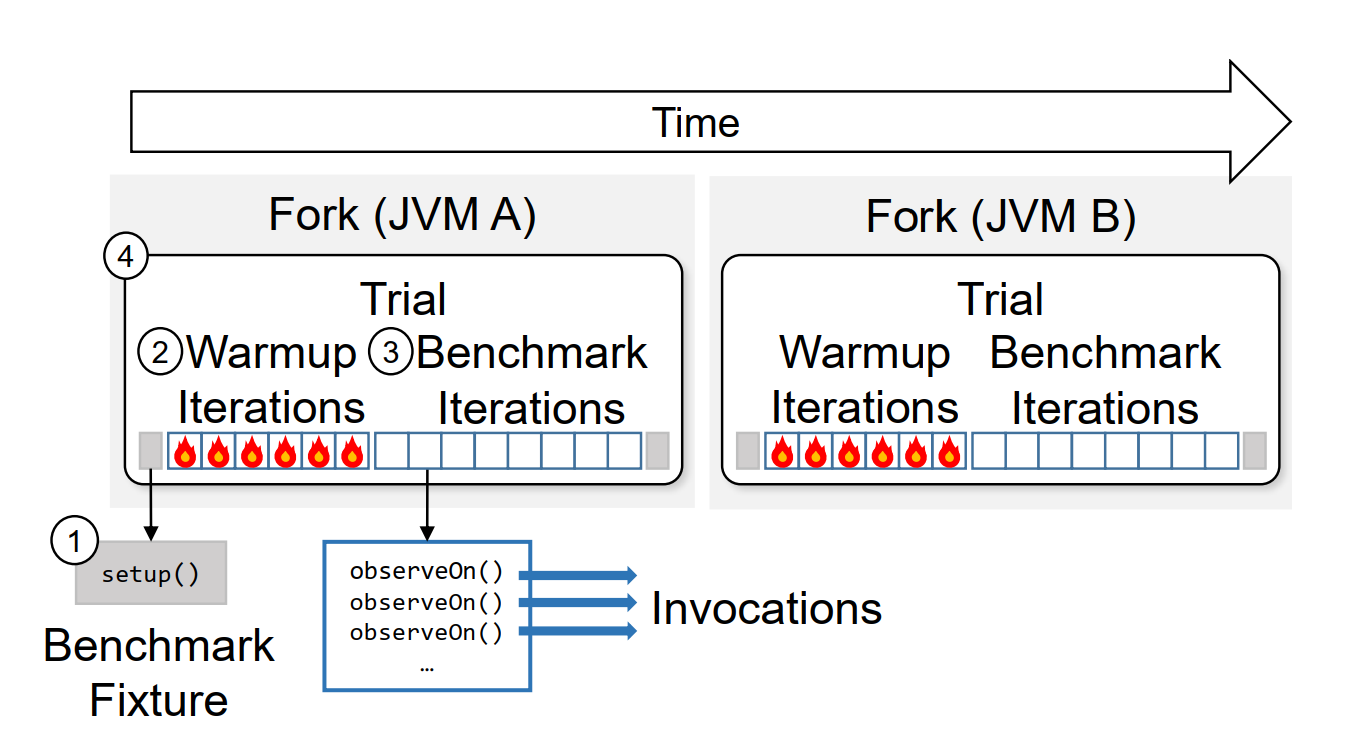
\includegraphics[width=\linewidth]{JMHBenchmark}
	\caption{Execution of a microbenchmark in JMH, taken from \cite{costa2019}.}
	\label{fig:JMHBenchmark}
\end{figure}

\noindent Depending on the underlying testing framework, developers can choose to run a benchmark for a limited time to see how many iterations can happen in this pre defined time, or also choose to run the benchmark for a specific amount of iterations to see how long it takes the functions within the benchmark to result in average. Such frameworks are especially useful for when determining whether a new introduced feature in the system causes performance regressions. Furthermore, these regressions can be detected early whilst still being in the development stage of the software, and according changes to the code can be scheduled before the changes go to production, which ensures the stability for the performance in the evolution of the software.


\subsection{Microbenchmark variability}

Unless otherwise configured, when a microbenchmark is run, it executes the underlying code for a certain time period (e.g., 1s) over and over for each benchmark iteration and returns a collection of average execution times for each benchmark iteration\cite{laaber2019software}. Execution times of a benchmark are usually expressed in nanoseconds \cite{laaber2019software} \cite{costa2019}. In this thesis, the term microbenchmark variability refers to the variability of a microbenchmark's resulting collection of execution times. It is basically computed by measuring how far the single execution times fall from the average execution time. In this manner, if the executions times are in the close neighborhood of the average value, the benchmark is considered as stable and it's predicted that another execution would take same or similar amount of nanoseconds as the average value. If, however, the points are distributed on a broader scale, it means that the benchmark is rather unstable, i.e., it cannot be predicted how long another execution of the benchmark will take.\\
\\
There are 2 main metrics that I use to calculate the variability of a microbenchmark in this thesis. The first one is called \textbf{coefficient of variation (CV)}, which is also known as the relative standard derivation\cite{laaber2019software}. "CV is a statistical measure for dispersion among a population of values" \cite{laaber2019software}, and in this thesis I use CV on the performance counters (i.e. average execution times in nanoseconds) of a microbenchmark's benchmark iterations to calculate the variation of a microbenchmark. CV is a measurement that is used to determine the variability in pervious studies as well \cite{laaber2019software} \cite{Leitner:2016:PCS:2926746.2885497}. Additionally, I calculate the \textbf{relative confidence interval width (RCIW)} with 95 and 99 percent confidence intervals of each microbenchmark and refer to them as RCIW95 and RCIW99 respectively. "The RCIW describes the estimated spread of the population's CV, as computed by statistical simulation"\cite{laaber2019software}.\\
\\
Regarding calculations of these metrics: CV is calculated by dividing the standard deviation of a dataset by the mean of the dataset. For RCIW, another methodology is followed, which is explained as bootstrapping with hierarchical random resampling and is also used in Laaber et al.'s paper \cite{laaber2019software}\cite{davison_hinkley_1997}\cite{hierach_data_2010} . The reason to follow this methodology resides in the non-normalized performance measurements \cite{laaber2019software}. Bootstrapping with randomly resampling refers to randomly sampling data points from a dataset, and in this thesis I use this technique with 10.000 bootstraps on the execution times of each microbenchmark to generate a collection of normalized mean values out of them, which I can then use to create the 95 and 99 percent relative confidence intervals.

\begin{figure}[H]
	\centering
	\begin{subfigure}{.5\textwidth}
		\centering
		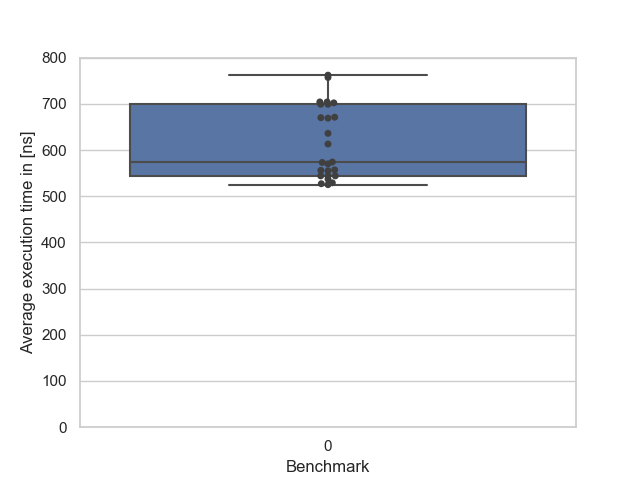
\includegraphics[width=\linewidth]{10percentvariance}
		\caption{Execution results of a microbenchmark with a RCIW99 of 10.28}
		\label{fig:10percentvariance}
	\end{subfigure}%
	\begin{subfigure}{.5\textwidth}
		\centering
		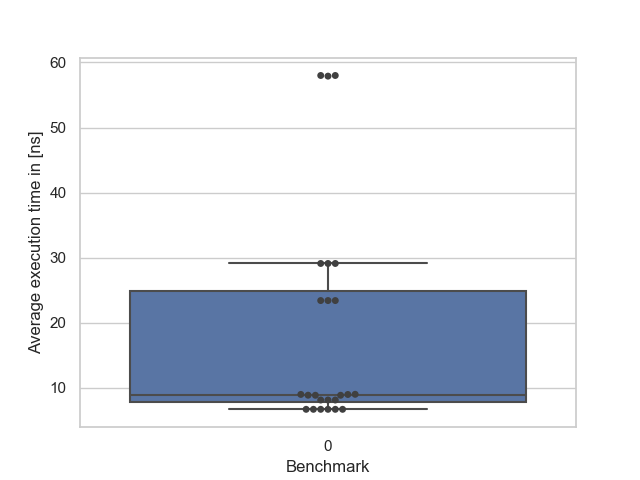
\includegraphics[width=\linewidth]{60percentvariance}
		\caption{Execution results of a microbenchmark with a RCIW99 of 64.18}
		\label{fig:60percentvariance}
	\end{subfigure}
	\caption{Example for a low and high variance microbenchmark}
	\label{fig:variances}
\end{figure}

\noindent To illustrate a low and high variable microbenchmark: Figure \ref{fig:10percentvariance} shows the execution times of the benchmark \textit{BenchmarkAddSafe} from \textbf{deckarep/golang-set} project\cite{deckarep/golang-set}. As the box plot shows, the points are all within the whiskers and there are no outliers. Also, the distribution of the points vary from 506 to 650 nanoseconds and it has a 99 percent confidence interval width (RCIW99) score of 10.28. In Figure \ref{fig:60percentvariance}, the benchmark \textit{BenchmarkParseUintHex} from \textbf{segmentio/objconv} project \cite{segmentio/objconv} is shown with its execution times. This benchmark's average execution times vary from 6.68 nanoseconds to 57.9 nanoseconds, having 3 outliers. This time, RCIW99 score is 64.18. The  score in RCIW99 is an estimator for the variability, hence, the higher this score, the higher variability the benchmark has.\\
\\
The variability of a benchmark may depend on a lot of factors such as the execution platform, the hardware the benchmarks are executed on, or, even the programming language of the microbenchmark itself\cite{laaber2018performance}. For example, the same benchmark can deliver different average values on different CPUs, as one CPU may perform much more operations in a second than the other one. Similarly, the same benchmark can have a different average for the execution time in a personal computer than the average in a cloud-based machine, or in different cloud-based machines compared to each other \cite{laaber2019software}. Some other factors include the concurrency, I/O latencies, virtualization etc.\\ \cite{laaber2019software}.
\\
Variability is a crucial factor of a benchmark, because it has an impact on the stability and reliability of it's results \cite{Laaber:2018:EOS:3196398.3196407}. It is important to have stable and reliable benchmarks, because then the developers can rely on the results of the microbenchmarks when they test parts of the software and find the regression causes with a higher trust. To this end, it's essential to predict the variability of microbenchmarks. There has been studies trying to predict the variability of performance tests in public Infrastructure-as-a-Service (IaaS) clouds by comparing aspects such as hardware heterogeneity, multi-tenancy and control over optimizations \cite{Leitner:2016:PCS:2926746.2885497}, or by comparing the outcomes of forks, trials and iterations in terms of variability \cite{laaber2019software}. One way to predict the variability might be through analyzing source code properties of the software. This can on one hand help the developers identify the cause of slowdowns in a newer version for example, on the other hand help them understand which source code property affects the results in which way.\\
\\
Executing usual performance tests (e.g., stress tests, load tests etc.) of a software is usually a long, time consuming process that can take up to days to finish\cite{Laaber:2018:EOS:3196398.3196407}. If a developer can rely on the microbenchmarks of the software, this can help reduce the time spent on performance tests for the whole project. When testing the software for performance via microbenchmarks, the aim of the developer is to have the highest possible coverage  with the minimal effort. For this, the minimal benchmark suite is needed, which should cover all or the most of the functionalities in the software. As the size of the software grows, the microbenchmark suite grows as well, and it gets harder to keep track of the tested and not tested functions. To this manner, the importance of predicting variability causes dives in. To keep the size of the benchmark suite minimal while having a good coverage, developers might not need testing all the functionalities. That's why, it's a good idea to predict which parts of the source code should be tested by predicting the variability of the benchmarks based on source code. With this, developers can be supported to write better benchmarks by for example being alerted to which new functions should have priorization in testing for performance.\\
\\
In this thesis, my aim is to find whether there is a correlation between the source code and the variability of a benchmark. For this, I analyze source code properties of microbenchmarks written in Go and use them as dependent variables of a statistical equation,  where the independent variable is the variability of the benchmark in RCIW99. The results can be used to understand the correlation between source code and variability, as well as be used to predict the variability of a benchmark for further applications.\\

\subsection{Go}


Go is a statically typed, compiled programming language, designed at Google and was released in November 2009 \cite{go}. Some of its innovational features include built-in data structures for advanced concurrent programming, Goroutines as lightweight processes and built-in performance benchmarking/testing libraries. While still being quite a new language among other languages, Go is the forth most active programming language in Github, and third-most highly paid language globally, according to Stack Overflow Developer Survey 2019\cite{stackoverflowdev}. Furthermore, it is effectively used in the industry and has a growing community.\\
\\
Go comes with a great built-in package for testing and benchmarking, which makes it easier for developers to unit test their code while still developing, or measure the performance of their functions\cite{gobench}. To create a benchmark function, the only thing one has to write is a function beginning with the name \textbf{"Benchmark"} and give a parameter \textbf{*testing.B}. These functions are typically defined in files ending with the \textbf{\_test.go} suffix, and the collection of all the benchmarks within a project build its microbenchmarking suite. Listing \ref{BenchmarkSrc} shows the example benchmark \textit{BenchmarkHash} from project \textbf{ironsmile/nedomi} \cite{ironsmile/nedomi}.


\begin{lstlisting}[caption=An example benchmark from \cite{ironsmile/nedomi}, label={BenchmarkSrc}, language=Go]
func BenchmarkHash(b *testing.B) {
	var m = buildMapHash(id, count)
	for i := 0; b.N > i; i++ {
		if _, ok := m[first.Hash()]; !ok {
			b.Fail()
		}
		if _, ok := m[middle.Hash()]; !ok {
			b.Fail()
		}
		if _, ok := m[last.Hash()]; !ok {
			b.Fail()
		}
	}
}
\end{lstlisting}

Go also supports these built-in packages with a CLI flag called "test", with which a developer can execute all the tests of a project on a single command. Executing all benchmarks takes an additional flag "bench", which executes all the benchmarks found in the current directory(package) of a project. An example run of a microbenchmark suite from \textbf{tidwall/buntdb} \cite{tidwall/buntdb} can be seen in Listing \ref{testbench}. The first column is the name of the benchmark, the second column is the amount of executions and the third column is the execution time per execution \cite{gobench}.

\begin{lstlisting}[caption=Example microbenchmark suite execution from \cite{tidwall/buntdb}, label={testbench}]
mikael@mikael-VirtualBox:~/Desktop/BenchmarkProjects/tidwall/buntdb/src-
/github.com/tidwall/buntdb$ go test -bench=.
goos: linux
goarch: amd64
pkg: github.com/tidwall/buntdb
Benchmark_Set_Persist_Random_1-4           	  300000	      4467 ns/op
Benchmark_Set_Persist_Random_10-4          	 1000000	      2094 ns/op
Benchmark_Set_Persist_Random_100-4         	 1000000	      1690 ns/op
Benchmark_Set_Persist_Sequential_1-4       	  500000	      3614 ns/op
Benchmark_Set_Persist_Sequential_10-4      	 1000000	      1388 ns/op
Benchmark_Set_Persist_Sequential_100-4     	 1000000	      1209 ns/op
Benchmark_Set_NoPersist_Random_1-4         	 1000000	      1774 ns/op
Benchmark_Set_NoPersist_Random_10-4        	 1000000	      1135 ns/op
Benchmark_Set_NoPersist_Random_100-4       	 1000000	      1107 ns/op
Benchmark_Set_NoPersist_Sequential_1-4     	 1000000	      1821 ns/op
Benchmark_Set_NoPersist_Sequential_10-4    	 2000000	       744 ns/op
Benchmark_Set_NoPersist_Sequential_100-4   	 2000000	       746 ns/op
Benchmark_Get_1-4                          	 2000000	       808 ns/op
Benchmark_Get_10-4                         	 3000000	       544 ns/op
Benchmark_Get_100-4                        	 3000000	       525 ns/op
Benchmark_Ascend_1-4                       	 5000000	       317 ns/op
Benchmark_Ascend_10-4                      	 2000000	       594 ns/op
Benchmark_Ascend_100-4                     	  500000	      3034 ns/op
Benchmark_Ascend_1000-4                    	   50000	     27257 ns/op
Benchmark_Ascend_10000-4                   	    5000	    271873 ns/op
Benchmark_Descend_1-4                      	 5000000	       304 ns/op
Benchmark_Descend_10-4                     	 3000000	       565 ns/op
Benchmark_Descend_100-4                    	  500000	      3065 ns/op
Benchmark_Descend_1000-4                   	   50000	     27362 ns/op
Benchmark_Descend_10000-4                  	    5000	    275479 ns/op
PASS
ok  	github.com/tidwall/buntdb	71.590s
\end{lstlisting}



\section{Related Work}
Here comes the literature research about benchmark variability. While some papers look at the benchmark variability causes, some of them try to predict the performance regressions based on different versions of a software by analyzing different commits and mining source code. \\
\\
To the best of my knowledge, there exist no study analyzing benchmark variability of software microbechmarks written in Go by trying to find a correlation with the used source code metrics in these benchmarks.\\
\\
Bunu duzelt
At the time of writing this thesis, most of the existing work is on the research of performance unit testing in Java ecosystem.\cite{Stefan:2017:UTP:3030207.3030226}
\cite{Laaber:2018:EOS:3196398.3196407}

\chapter{Methodology}
\label{Methodology}
In this section, I present the methodologies I followed to get to the results. As the project consists of 3 main steps, these steps are explained respectively.
\section{Calculating variabilities}
First part of the study involved doing a quantitive analysis by analyzing the given data set. From this data set, I firstly had to extract the valid projects, i. e. choose the projects that have a positive average benchmark score. Secondly, I calculated some metrics for each of benchmark that indicate the variability. The results follow in the first point of Results section.
\subsection{Data set}
The starting point was a data set that was acquired by Laaber et. al from a previous study? (Ask for details) \\
\\
Out of 482 projects, 230 of the projects qualified because they had a score bigger than -1 in the main file of data set. ...
\\
 This includes the categorization of benchmarks of 228 projects written in Go by looking at the total executions, the mean, coefficient of variation and relative confidence interval width with 95\% and 99\% confidence intervals. Secondly, we introduce the methodology we used to extract source code properties from in the first place chosen benchmarks. Thirdly, comparing the source code properties with the variabilities of benchmarks by using regression models to achieve the results.
 
\subsection{Metrics as the variability indicators}
For calculating the variabilities of benchmarks, I oriented myself at 3 main metrics. First metric is "Coefficient of Variation" (CV), which is a metric used often in statistics to calculate variability of a data set. ...

\subsection{Python coding}
How I coded the calculations and created the visualizations. \\
Which library I used for creating the visualization? \\
How I used the pa-tool to get the RCIW95 and RCIW99 values \\

\section{Extracting source code properties}
Second part of the study was to extract the source code properties of benchmarks written in Go. This also had 2 parts. Results of this part are to be found in second part of the Results section.

\subsection{Decision on source code properties}
Which steps I took at deciding for the source code properties

\subsection{Golang coding}
- How I coded in Go to extract the properties? (Also get into detail about AST's in Go and giving code examples) \\
- Which libraries or other tools I used (Callgraph tool, cyclomatic complexity tool) ? \\

\section{Finding correlations}
Third and last part of the study was to find correlations between source code properties of benchmarks and their variability. In this last part, I used a regression model on some chosen benchmarks to find correlations. Results of this part are to be found in the third part of Results section.
\subsection{First analysis - Second analysis}
- Which dependent and independent variables do I have for the comparison?
\subsection{Regression model}
- Which regression model I used for the results, how did I get the correlations results?

\section{Threats to the validity}
There are threats to the validity of this study.
\subsection{Number of projects}
There are probably thousands of projects written with Go. These can be with or without benchmarks, however, I was limited to a number of projects for the outcome of this study and the number might not reflect the truth.

\subsection{Chosen properties}
I presented my chosen properties for this analysis, however, are these enough for this study? There may be other metrics that might be very relevant to this study, which I haven't discovered whilst searching.

\subsection{Analysis of the unknown}
Since the analysis is made statically for the second part of the methodology, this can be a threat to the validity since we don't actually know which nodes in the cyclomatic complexity are visited.


\chapter{Results}
\label{Results}
In this section, I present the results from the 3 parts of this study. 
\section{Variabilities of benchmarks}
After calculating the variability metrics of benchmarks from the projects, I categorized the variabilities in 10 percent buckets starting from 0 o 100 percent. All the benchmarks that have a variability higher than 100 percent fall into one final bucket. ...

\section{Source code properties}
For every project that I was able to analyze by using the tool introduced in second part of methodology section, I was able to collect the source code properties. CSV? ...

\section{Correlation between variabilities and source code properties}
- Yes \\
- No \\
- Not really? \\
- Can't really say \\


\chapter{Discussion}
\label{Discussion}
In this section, I discuss the results that I obtained and how relevant these are.
\section{Chosen properties}
Do the chosen properties make sense? \\
Why did I choose these properties and how could these affect the benchmark variability? \\

\section{Static analysis}
This study involved doing a static analysis for the source code of project written in Go. What pros and cons does this have? Why doing a dynamic analysis would make more sense?

\section{Size of data set}
Coming from 482 open source projects written in Go, down to 228 that I could analyze. Is the size of data set small or big enough to acknowledge the results?

\section{Future Work}
What could be done with the results in this thesis in the future?

\chapter{Conclusion}
\label{Conclusion}
I finally conclude with what I have done with this project: How I started, which steps I took and which results I achieved.



\appendix
\chapter{First Append}




\backmatter



\bibliographystyle{ieeetr}
\bibliography{literature}

\end{document}
